% Created 2017-12-06 Wed 11:31
\documentclass[presentation]{beamer}
\usepackage[utf8]{inputenc}
\usepackage[T1]{fontenc}
\usepackage{fixltx2e}
\usepackage{graphicx}
\usepackage{longtable}
\usepackage{float}
\usepackage{wrapfig}
\usepackage{rotating}
\usepackage[normalem]{ulem}
\usepackage{amsmath}
\usepackage{textcomp}
\usepackage{marvosym}
\usepackage{wasysym}
\usepackage{amssymb}
\usepackage{hyperref}
\tolerance=1000
\usepackage{graphicx} \DeclareMathOperator{\argmin}{argmin}
\usetheme{simple}
\usecolortheme{}
\usefonttheme{serif}
\useinnertheme{}
\useoutertheme{}
\author{Talon Chandler}
\date{December 6, 2017}
\title{Update On 3D Orientation Reconstruction}
\hypersetup{
  pdfkeywords={},
  pdfsubject={},
  pdfcreator={Emacs 25.3.1 (Org mode 8.2.10)}}
\begin{document}

\maketitle
\begin{frame}[label=sec-1]{Spheroid Distribution}
\vspace{-1em}
\begin{center}
  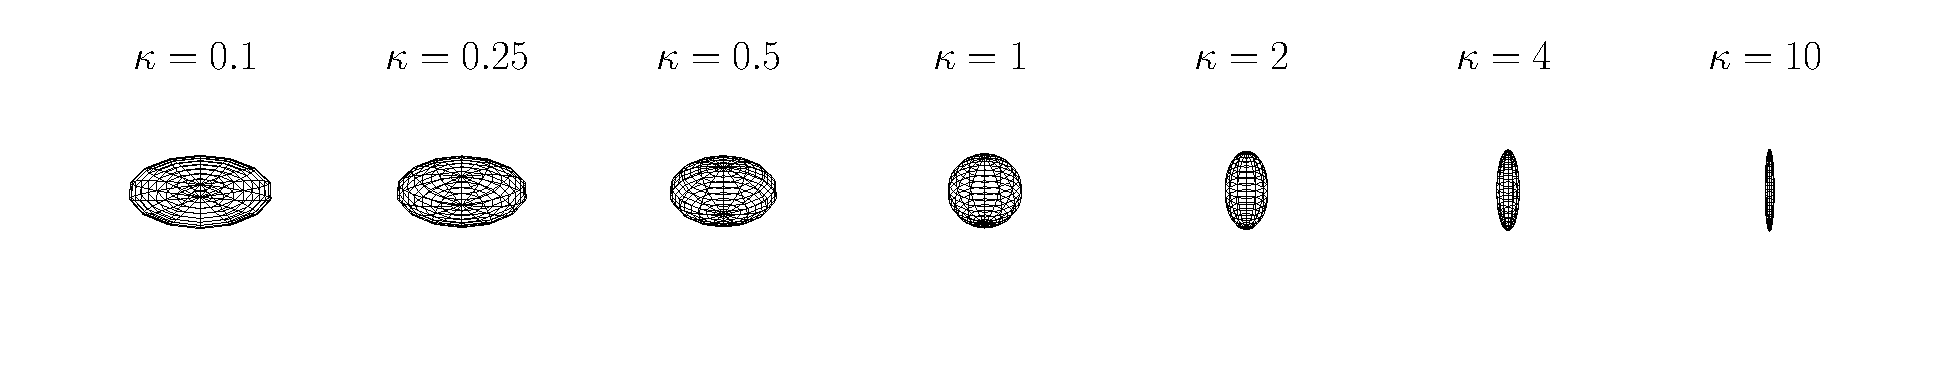
\includegraphics[width=1.0\textwidth, interpolate=true]{figs/spheroid.pdf}
\end{center}
\vspace{-4em}
\begin{align*}
  f(\vec{r}; \mathbf{A}) &= \frac{r^T\mathbf{A}^{-1}r}{|\mathbf{A}|}\\
  f(\vec{r}; \vec{r}', \kappa) &= \frac{\kappa}{S(\kappa)\sqrt{1+(\vec{r}\cdot\vec{r}')^2\left(\frac{1}{\kappa^2} - 1\right)}}\\
  S(\kappa) &= 2\pi\left(1 + \frac{\kappa^2}{2\sqrt{1-\kappa^2}}\log\left[\frac{1+\sqrt{1-\kappa^2}}{1-\sqrt{1-\kappa^2}}\right]\right)
\end{align*}
\vspace{-1em}
\begin{itemize}
\end{itemize}
\end{frame}
\begin{frame}[label=sec-2]{Forward Model: Single diSPIM Frame}
\begin{align*}
  \text{Measured Intensity:   }& I = \int_{\mathbb{S}^2}d\vec{r}\ I^s(\vec{r})f(\vec{r}; \vec{r}', \kappa)\\ \\
  \text{Single Fluorophore:   }& I^s(\vec{r}) = 2[A+B(1 - \cos^2\phi\sin^2\theta)]\times \\ & \hspace{7em}\sin^2\theta\cos^2(\phi - \phi_{\text{pol}})\\ \\
  \text{Spheroid Distribution:   }& f(\vec{r}; \vec{r}', \kappa) = \frac{\kappa}{S(\kappa)\sqrt{1+(\vec{r}\cdot\vec{r}')^2\left(\frac{1}{\kappa^2} - 1\right)}}
\end{align*}
\begin{itemize}
\item No luck integrating in closed form ;(
\end{itemize}
\end{frame}
\begin{frame}[label=sec-3]{Integrating Faster With Spherical Quadrature}
\begin{center}
  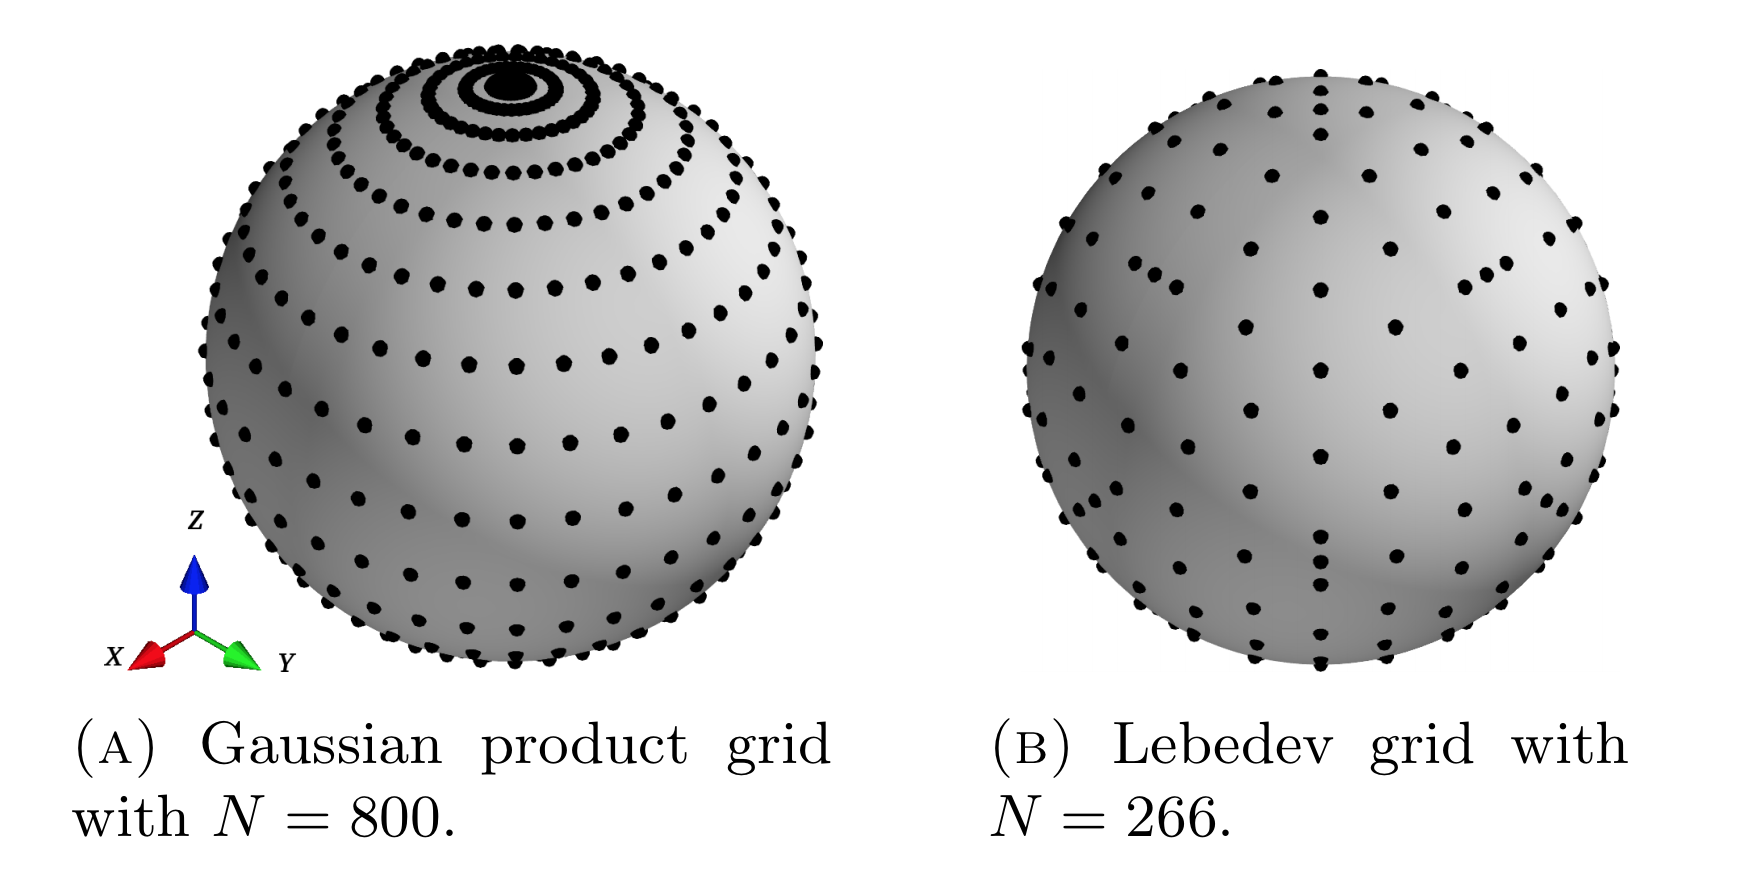
\includegraphics[width=0.7\textwidth, interpolate=true]{figs/quadrature.png}
  \raisebox{-10pt}{\makebox[0pt][r]{\footnotesize Beentjes, 2012}}
\end{center}
\begin{itemize}
\item Instead of evaluating integrals one after the other and using Gaussian quadrature (left), evaluate the integral all at once using Lebedev quadrature (right)
\item How many grid points do I need to use to accurately integrate?\\ To within 1\%? Perfectly? $\rightarrow$
\end{itemize}
\end{frame}
\begin{frame}[label=sec-4]{Harmonic Analysis On The Sphere}
\begin{align*}
  \text{Measured Intensity:   }& I = \int_{\mathbb{S}^2}d\vec{r}\ I^s(\vec{r})f(\vec{r})
\end{align*}
\begin{itemize}
\item Rewrite $I^s(\vec{r})$ and $f(\vec{r})$ in terms of orthogonal spherical harmonics\\ \\
\item Expensive integral becomes a cheap dot product of coefficients\\ \\
\item With measurements under different polarization settings we get $\vec{g} = \mathcal{H}\vec{f}$ where $\vec{g}$ is a vector of intensity measurements, $\vec{f}$ is a vector of spherical harmonic coefficients of the fluorophore distribution, and the rows of $\mathcal{H}$ are the spherical harmonic coefficients of $I^s(\vec{r})$ for each measurement \\ 
\item Null space of $\mathcal{H}$ corresponds to symmetries/degeneracies
\end{itemize}
\end{frame}
\begin{frame}[label=sec-5]{Harmonic Analysis}
\begin{itemize}
\item Harmonic analysis on $\mathbb{R}^n \rightarrow$ $n$-D Fourier Transform\\
\item Harmonic analysis on $\mathbb{S}^1$ (circle) $\rightarrow$ Fourier Series\\
\item Harmonic analysis on $\mathbb{S}^2$ (sphere) $\rightarrow$ 2D Fourier Series
\end{itemize}
\end{frame}
\begin{frame}[label=sec-6]{Spherical Harmonics}
\begin{center}
  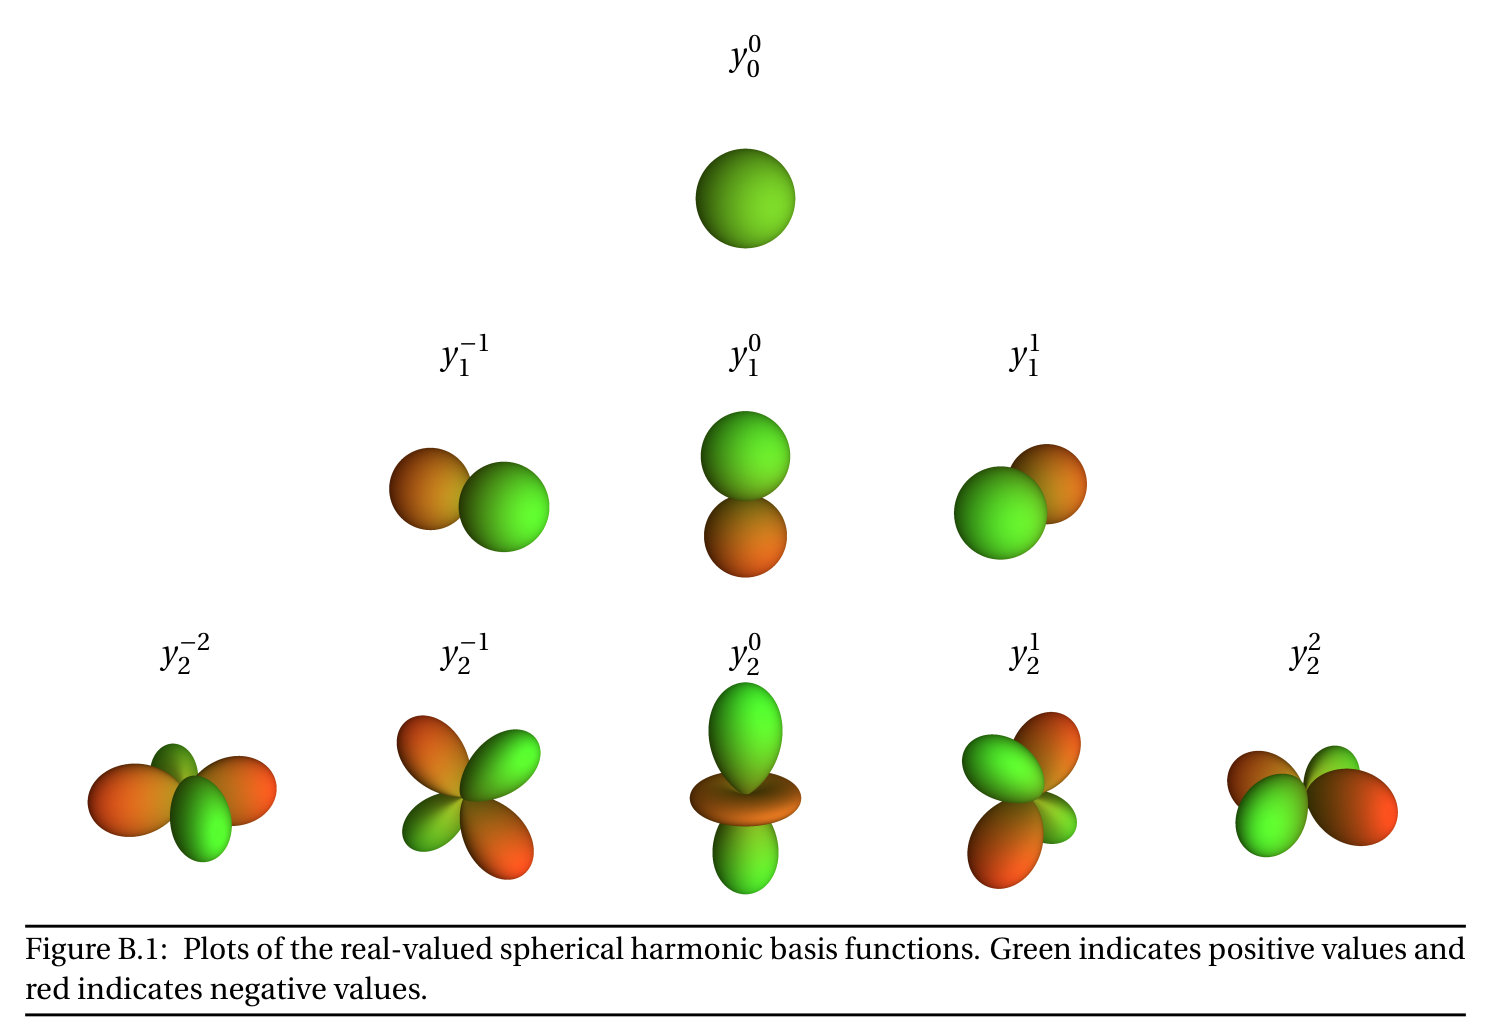
\includegraphics[width=0.9\textwidth, interpolate=true]{figs/harmonics.png}
  \raisebox{-10pt}{\makebox[0pt][r]{\footnotesize Jarosz, 2008}}
\end{center}
\end{frame}

\begin{frame}[label=sec-7]{Single View diSPIM Frame}
\begin{center}
  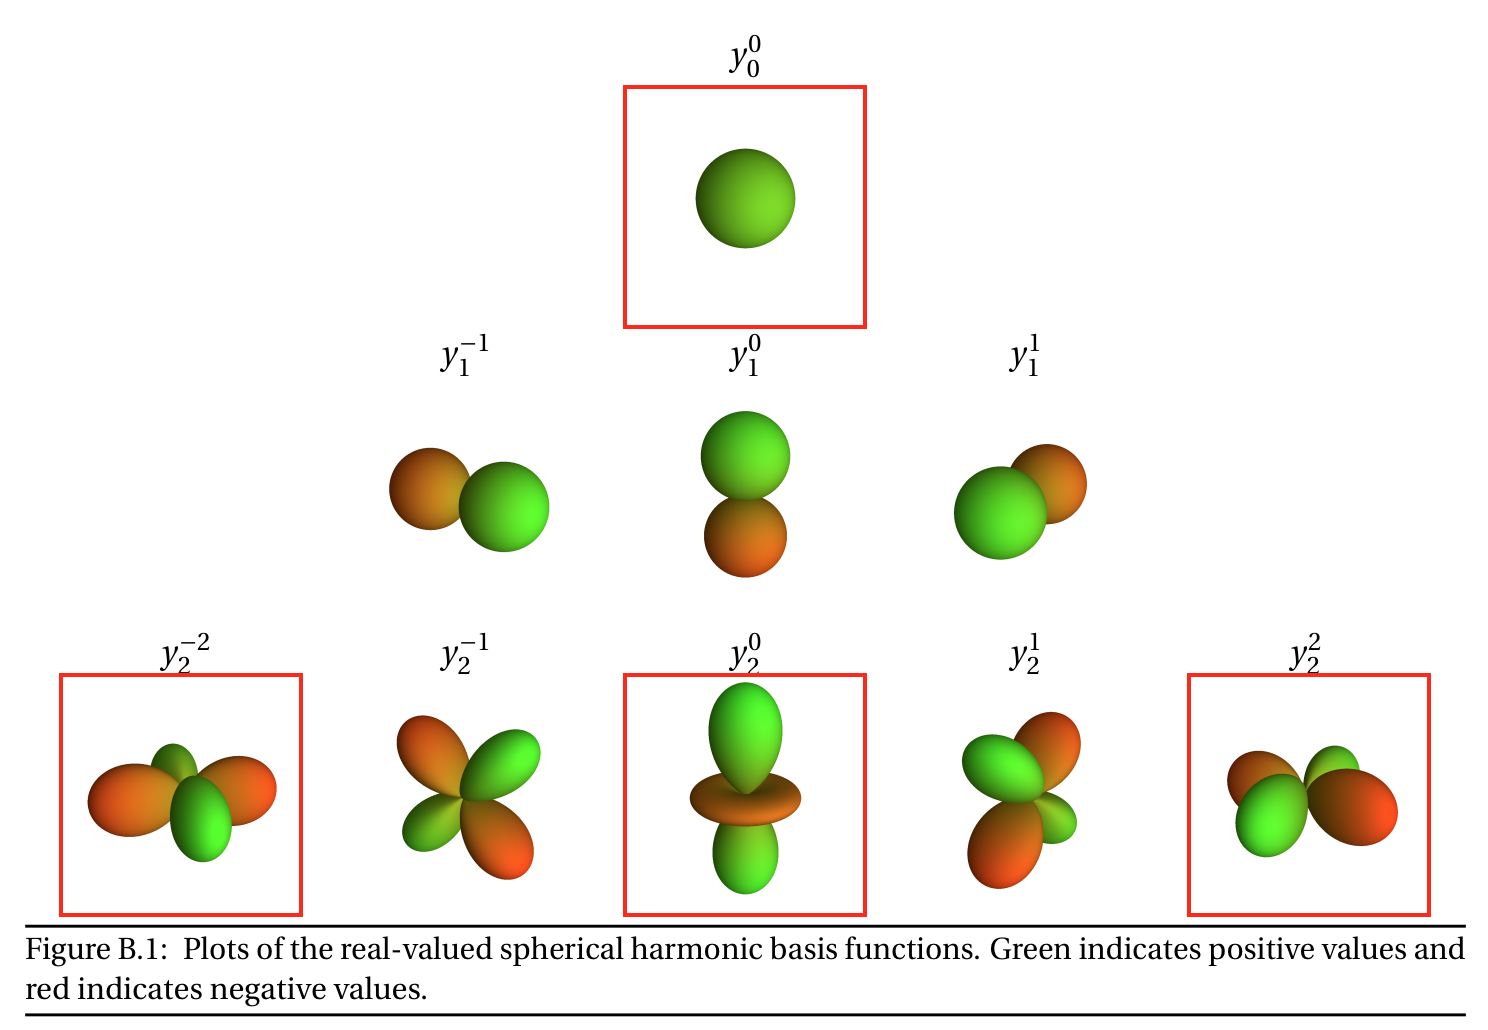
\includegraphics[width=0.7\textwidth, interpolate=true]{figs/harmonics_supp.png}
  \raisebox{-10pt}{\makebox[0pt][r]{\footnotesize Jarosz, 2008}}
\end{center}
\begin{itemize}
\item Non-zero coefficients for single view diSPIM frame shown in red boxes
\end{itemize}
\end{frame}
\begin{frame}[label=sec-8]{Early Conclusions + Upcoming Work}
\begin{itemize}
\item Odd bands aren't antipodally symmetric so they aren't present in the sample.
\item Zero coefficients on $y_2^{\pm 1}$. Corresponds to degeneracy? Investigating. 
\item Adding polarizers on the detection side with give us access to 4th order band. Still investigating degeneracy. 
\item A single fluorophore has non-zero components in all even bands (sort of like FT of $\delta(x)$ is 1). We can only measure the first few bands which constrains the accuracy of our estimates. 
\item Now we're estimating spherical harmonic coefficients instead of parameters of a hypothesized distribution. That's all of the info we can access. 
\item Upcoming---reconstruction in terms of matrix inversion! 
\end{itemize}
\end{frame}
% Emacs 25.3.1 (Org mode 8.2.10)
\end{document}